\documentclass[12pt,a4paper]{article}
\usepackage{amsmath,amsthm,amssymb,graphicx,hyperref}
\usepackage{float}
\usepackage[left=1.2in,right=1in,top=1in,bottom=1in]{geometry}
\usepackage[romanian]{babel}
\usepackage{mathtools}
\usepackage{indentfirst}
%\usepackage{...insert other packages here...}
\newtheorem{thm}{Teorema}[section]
\newtheorem{lem}[thm]{Lema}
\newtheorem{cor}[thm]{Corolarul}
\newtheorem{prop}[thm]{Propozi\c tia}
\theoremstyle{definition}
\newtheorem{defn}{Defini\c tia}[section]
\theoremstyle{remark}
\newtheorem{rem}{Remarca}[section]
\newtheorem{exmp}{Exemplul}[section]
\begin{document}
\thispagestyle{empty}
\begin{center}
\begin{figure}[h!]
\vspace{-20pt}
\begin{center}

\includegraphics[width=100pt]{FMI-03.png}
\end{center}
\end{figure}


{\large{\bf UNIVERSITATEA DE VEST DIN TIMI\c SOARA

FACULTATEA DE MATEMATIC\u A \c SI INFORMATIC\u A

PROGRAMUL DE STUDII DE LICEN\c T\u A : Informatic\u a  }}

\vspace{120pt}
{\huge {\bf LUCRARE DE LICEN\c T\u A}}

\vspace{150pt}
\end{center}

{\large\noindent{\bf COORDONATOR:\hfill ABSOLVENT:}

\noindent Conf. Dr. Marc Frîncu \hfill Andrada Lorena Sandu}

\vfill
\begin{center}
{\bf TIMI\c SOARA

2021}
\end{center}
\newpage
\thispagestyle{empty}
\begin{center}
{\large{\bf UNIVERSITATEA DE VEST DIN TIMI\c SOARA

FACULTATEA DE MATEMATIC\u A \c SI INFORMATIC\u A


PROGRAMUL DE STUDII DE LICEN\c T\u A : Informatic\u a  }}

\vspace{120pt}
{\huge {\bf Analiza pădurilor și a apelor folosind tehnici de observare a Pământului}}

\vspace{150pt}
\end{center}

{\large\noindent{\bf COORDONATOR:\hfill ABSOLVENT:}

\noindent Conf. Dr. Marc Frîncu \hfill Andrada Lorena Sandu}

\vfill
\begin{center}
{\bf TIMI\c SOARA

2021}
\end{center}
\newpage
\section*{\bf Astract}

Climate change has become in recent years one of humanity's foremost problems. However, accessible information is still scarce. We will attempt
 to analyze satellite images in order to detect forests and bodies of water, as these are the easiest to recognize.
 
 
 To achieve this, we developed a plugin for the Qgis application, in order to better detect the events that lead up to changes in forests and waters.
 These can be highlighted using certain formula that help us quickly identify these changes and, therefore, assist us in reacting faster to such events.
 
 
 The plugin we developed uses the NDVI(Normalized difference vegetation index) and NDWI(Normalized difference water index) on the generated images to improve the efficiency
 of analyzing such images.
 
 \newpage
 \section*{Abstract}
 
Schimbările climatului au devenit în ultimi ani o problemă majoră în viață oamenilor.Accesul la informațiile despre acestea încă este limitat.
Vom analiza cu ajutorul imaginilor satelitare, într-un mod util, pădurile și apele.

Pentru a realiza acest lucru, am dezvoltat un plugin pentru aplicația Qgis, pentru a detecta mai bine evenimentele care duc la schimbările legate de suprafețele  pădurilor și a apelor. Acestea pot fi evidențiate folosind anumite formule care ne ajută să identificăm rapid aceste schimbări și, prin urmare, ne ajută să reacționăm mai rapid la astfel de evenimente.


Acest plugin folosește formula pentru NDVI(Indicele de diferență normalizată a vegetației) și NDWI(Indicele de diferență normalizată a apei) pentru a putea  eficientiza generare unei analize mai clare prin imaginile satelitare.
\markright{}
\newpage
\normalsize{}
\tableofcontents
\newpage
\section*{\bf Capitolul 1}
\markright{}
\section*{{\bf Introducere}}
\markright{}
\addcontentsline{toc}{section}{Intoducere}
\setcounter{section}{1}
\subsection{{Motiva\c tie}}

Laurent Clerque spunea că pentru ca ființele umane să își ridice picioarele acestea trebuie să sfideze gravitația.Încă de la începutul timpurilor inovația a fascinat întreagă lumea. Această creare a început în  secolul al XVII-lea când cei doi frați Montgolifer au lansat primul balon cu aer cald sper cer,acesta având să fie folosit de armata franceza în scopuri militare. Dar pe parcusul timpului inventatori doreau să creeze ceva mai bun ,de aceea la sfârștiul secolului al XIX-lea francezul Gustave Hermite a invetat “sound balloon” . Aceste baloane meteorologice au devenit utile cu timpul,din cauza dezvoltări transmițătorilor  radio. În anul 1930 aceștia permiteau transmiterea datelor în timp real . Din cauza performantei pe care au dovedit-o ,transmițătorii au fost montați pe aeronave,astfel încât acestea să poate efectua inspecții zilnice \cite{istorie} \cite{istorie2}.


Institutul Național Geografic din Franța folosea fotografiile aeriene ,atunci când aceștia își creau hărțile,desigur tot în scopuri militare. Aceste documente fiind folosite și astăzi la drumeții și consili locale.Aceste acte sunt cu adevărat valoroase  atunci când ,sunt actualizate în mod regulat. Întrucât acestea, în funcție de fenomele naturii care se produc ,se pot schimba . În concluzie observarea pământului poate fi unul dintre beneciciile cheie ,alea oamenilor de știință ,a proiectelor și experimentelor pe care aceștia doresc să le producă \cite{istorie} \cite{istorie2}.


Sputnik a fost primul satelit care în anul 1957 orbita în jurul Pământului. Acești sateliți au mai multe roluri importante,cum ar fi: telecomunicații,geolocalizare/navigația și observarea Pământului. Întrucât planeta Pământ este de natura sferica cartografia a fost și este o disciplina extrem de tehnica,deoarece imaginile trebuie mereu aplatizate și asamblate într-un mozaic concret \cite{wikisputnik}.


De asemenea în zilele noastre sateliți care orbitează în jurul planetei sunt mulți și de tipuri diferite. Sateliții astronomici, biosateliți,sateliți de comunicații,sateliți de observare,sateliții de navitagatie sunt doar o parte din sateliți care orbitează în jurul planetei \cite{wikisputnik}.


Sateliți pe care ne bazam în aceasta lucrarea de licență sunt sateliți de observare care  colectează   informații despre sistemele fizice ,biologice și chimice ale planetei Pământ prin intermediul tehnologiilor de teledetecție. Aceasta colectare , de obicei, implica sateliți care transporta dispozitile de imagistica.Aceasta metoda este folosita cu scopul de a monitoriza și evalua starea ,dar și modificările mediului înconjurător. cite{istorie} \cite{istorie2}.Tehnologiile spațiale oferă o mare varietate de seturi de date fiabile,astfel acestea putând fi combinate cu cercetare și dezvoltarea metodelor adecvate și cerute de către cercetători. Prin acest mod oferind un mijloc unic de coletare și procesare a datelor referitoare la planeta \cite{wikisputnik}.

SENTINEL-2 este un satelit care orbitează în jurul planetei Pământ. Acesta a fost lansat ca partea a programului “Copernicus” pe 23/06/2015 . Aceste satelit este special ,întrucât este conceput în mod special pentru a furniza o multitudine de date ,dar și de imagini satelitare. SENTINEL-2 este echipat cu un sensor multispectral opto-electric pentru supraveghere cu o rezoluție de la 10 până la 60 m,în zonele vizibile ,în infraroșu apropiat (NIR) și infraroșu cu unde scurte (SWIR) ,inclusive 13 canale spectrale ,care asigura captarea diferențelor în stare de vegetație etc. Orbita are o înălțime medie de 785 km \cite{wiki}.


Motivația pe care eu am avut-o în momentul în care am decis să aleg aceasta lucrare de licență este aceea de a cunoaște mai bine ceea ce ne înconjoară . Întrucât suntem în momentul în care tehnologia este parte din viață noastră,iar accesul la informație este la un click distanță. Cunoașterea și învățarea sunt anumite funcții vitale,pentru ca noi să putem progresa. 
 

\subsection{{Scurt\u a prezentare a temei propuse}}

Lucrarea aleasă se bazează pe analiza astreonomică care va prelua și va prelucra imagini satelitare,bazîndu-se pe cele trei benzi de culoare (verde,roșu,albastru)pe care  acestea le au. Rezultatul dorit fiind o detecție pe baza acestor imagini. Detecția se va face pe zone precum:păduri și ape.Toate acestea în scopul evidențierii acestor zone într-un mod mult mai rapid, darîn același timp și mai plăcut.


Este simplu de observat liber apele și pădurile pe o harta.Modul de a detecta se schimba drastic atunci când nu ochiul uman detectează ,ci o tehnologie.Scopul acestei lucrări este de a dezvolta o aplicație care nu este de sine stătătoare,ci mai degrabă de a dezvolta un plugin care să lucreze împrepuna cu Qgis pentru a putea beneficia de toate avantajele și pentru a putea aduce noi funcționalități.Acest lucru făcând posibil prelucrarea ,importarea și afișarea imaginilor satelitare.

Revenind din nou la benzile de culoare din care sunt formate imaginile satelitare ,prin prelucrarea imaginilor înțelegem capacitatea scriptului de a citi valorile benzilor respective și folosind anumite formule matematice să reproducă imaginea inițială într-un mod în care zonele dorite de utilizator să fie evidențiate și mult mă ușor observabile.


Acest plugin în principal va avea nevoie de o interfață grafică pentru ca utilizatorul să poată să interacționeze și să prelucreze acestea imagini. Interfață grafica va fi una ușor de înțeles cu un stil minimalist ,dar și intuitiva pentru ca utilizator să înțeleagă mai ușor ceea ce poate să dezvolte pornind de la acest script.Prin accesarea mai multor butoane și alegerea de zone geografice pe care le dorește,acesta poate să importe ,să prelucreze și să exporteze imaginile dorite într-un mod mult mai intuitiv și mai bine concrentizat. 


\subsection{{Solu\c tii si abord\u ari similare}}

O aplicatie similara este "FSC GIS Portal". 

"FSC GIS Portal" este o aplicație web geospatiala pentru utlizarea voluntara de către auditorii de gestionare a pădurilor din întreagă lume.Aceasta permite oamenilor să observe  evoluția și modificările aduse acestei păduri în timp. Aplicația este capabila fie să își actulizeze datele despre o anumită locație complet automat,pe baza imaginilor satelitare fie se poate folosi de date suplimentare oferite de către personale care au fost responsabile de gestionarea zonei pentru a oferi o analiz\u a mai detaliat\u a. În prezent aceasta aplicație este limitata de autoritățile certificate \cite{aplicati}.




\newpage
\section*{\bf Capitolul 2}
\markright{}
\section*{{\bf Structura}}
\markright{}
\addcontentsline{toc}{section}{Structura}
\setcounter{section}{1}
\refstepcounter{section}{}
\subsection{Imagini Satelitare}
 Imaginile satelitare ne oferă informați despre Pământ în fiecare minut. Imaginile prin satelit sunt imagini ale Pămîntului sau ale altor planete colectate de către sateliții si preluate de către guverne și companii din întreaga lume. \cite{wiki} Primele fotografii prin satelit  ale Pământului au fost făcute in 14 august 1959 de US Explorer 6. Primele imagini satelitare ale Lunii au fost făcute la 6 octombrie 1959 de satelitul sovietic Luna 3 \cite{satelitare}.
\subsection{Rezoluția}
Atunci când lucram cu imagini din satelit, rezoluția are un rol important.Există patru tipuri de rezoluții: radiometrică, temporală, spectrală, spațială.

\subsubsection{Rezoluția radiometrică}

Rezoluția radiometrică reprezintă capacitatea unui senzor digital de a distinge valorile de gri.\cite{radiometrica} Un satelit percepe diferite unde de lumini la anumite intensități. Aceasta poate să distingă doar între lumina si întuneric \cite{radiometrica}.

\subsubsection{Rezoluția temporală}

Rezoluția temporală oferă informații despre disțanta dintre două imagini satelitare din aceeași zona.Cu cât aceasta este mai mare cu atât este mai mica distanța de timp dintre imaginile satelitare. De asemenea, mai multi sateliți au o rezoluție temporală în medie de 14 zile.Satelitul SENTINEL 2A captează imagini din acelasi punct la 5 zile distanță \cite{temporala}.

\subsubsection{Rezoluția spectrală}

Senzorii spectrali de satelit percep Pământul ca find gri. Acest lucru se datorează faptului ca fiecare senzor detectează fiecare lungime de unda separat prin benzile spectrale. Cu cât numarul de benzi al unui senzor este mai mare, cu atât este mai mare si rezoluția spectrală a unui satelit \cite{temporala}.
 
\subsubsection{Rezoluția spațială}

Rezoluția spațială  este evaluată prin cât din imaginea reprezintă un pixel, ceea ce oferă detaliile sale.

Satelitul Landsat 8 este echipat cu doi senzori, Operational Land Imager (OLI) și senzor termic cu infraroșu (TIRS)\cite{spatiala}. Aceste doi senzori asigură acoperire la o rezoluție spațială de \cite{spatiala}:

\begin{figure}[H]
  \centering
  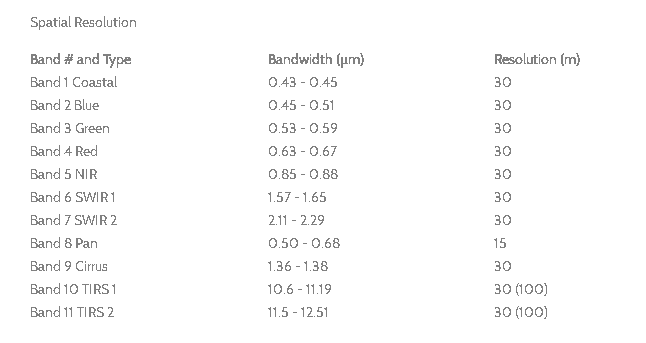
\includegraphics[width=400pt]{landsatspatial2.PNG}
  \caption{Rezoluția spațială LANDSAT 8 \cite{spatiala}}   
\end{figure}

• 15 metri: pancromatic;

• 30 de metri: vizibil, NIR, SWIR;

• 100 de metri: termic.

Satelitul Sntinel 2A asigură acoperirea la o rezoluție de \cite{spatialasentinel}
\cite{spatialasentinel2}: 


\begin{figure}[H]
  \centering
  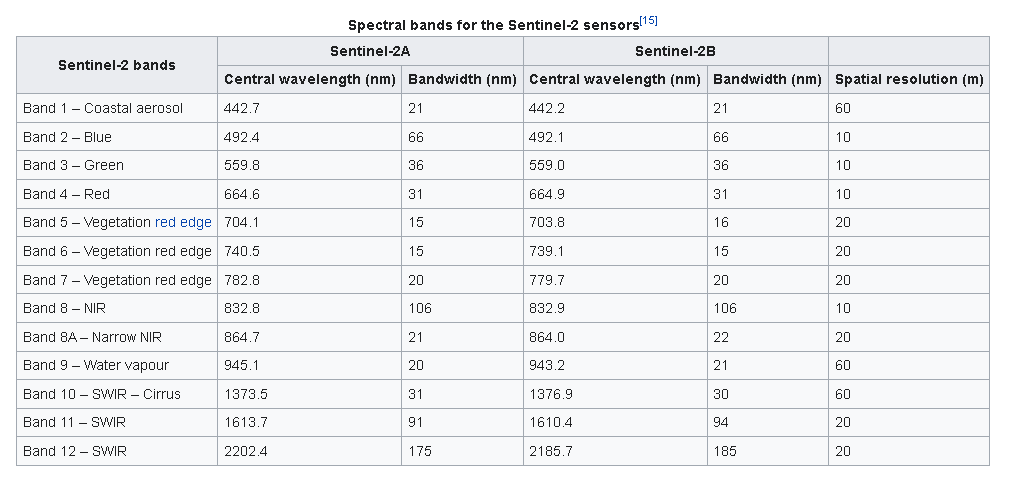
\includegraphics[width=400pt]{sentinelspatial.PNG}
  \caption{Rezoluția spațială SENTINEL 2A \cite{spatialasentinel}}   
\end{figure}

• 10 metri: visible, VNIR;

• 20 metri: visible, VNIR, SWIR;


• 60 metri: visible, VNIR, SWIR. 


\subsection{LANDSAT 8}
\subsubsection{Despre Landsat 8}


Landsat 8 este un satelit american de observare a Pământului lansat la 11 februarie 2013. Este al optulea satelit din programul Landsat. Denumit inițial Landsat Data Continuity Mission (LDCM), este o colaborare între NASA și Studiul Geologic al Statelor Unite (USGS).  Acesta cuprinde Operational Land Imager (OLI) și senzorul termic cu infraroșu (TIRS), care poate fi utilizat pentru a studia temperatura suprafeței Pământului și este utilizat pentru a studia încălzirea globală \cite{ladsat}.

Satelitul a fost construit de Orbital Sciences Corporation, care a servit ca prim contractor pentru misiune. În primele 108 de zile pe orbită, LDCM a fost supus controlului și verificării de către NASA, iar la 30 mai 2013 operațiunile au fost transferate de la NASA către USGS când LDCM a fost redenumit oficial în Landsat 8 \cite{ladsat}.

\begin{figure}[H]
  \centering
  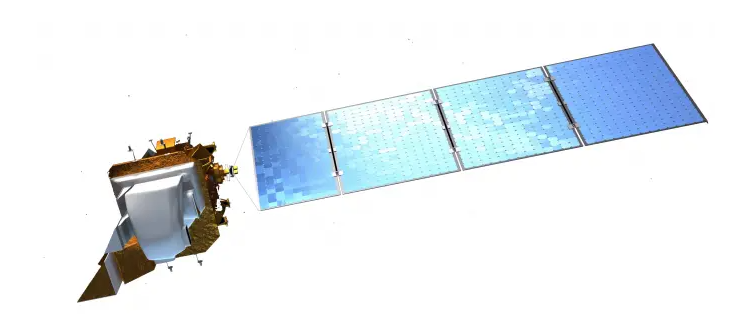
\includegraphics[width=400pt]{LANDSAT8.PNG}
  \caption{Satelitul Landsat 8 \cite{landsat8} }   
\end{figure}
\subsubsection{Landsat 8 benzi spectrale}


Benzile Landsat 8 sunt imagini de tip TIFF cu o rezoluție între 7000 și 8000 pixeli,
cu 1 pixel reprezentând 30 de metri. O scenă acoperă aproximativ 210 km și este actualizată la
la fiecare 16 zile. Adâncimea de biți a imaginilor este de 16 . Pentru această lucrare am luat în considerare doar benzile patru(RED) și cinci(NIR), întrucât acestea o să ne ajute la calcul indicelui de vegetație.



\subsubsection{Benzile spectrale RED și NIR}

Banda spectrala RED este o culoare tradițională, întrucât face parte din grupul rgb(red,green,blue)și face partea din 'Natural Color Image'. Cu aceste benzi sunt generate imagini care au aspectul cel mai apropiat de o imagine reala.


Banda spectrala NIR măsoară infraroșul apropiat. Această parte a spectrului este deosebit de importantă pentru ecologie, deoarece plantele sănătoase o reflectă - apa din frunzele lor împrăștie lungimile de undă înapoi în cer. În comparație cu alte benzi, obținem indici precum NDVI, care ne permit să măsurăm sănătatea plantelor \cite{rednir}.

Aceste doua benzi au ca și secificații:

\begin{table}[ht]
\caption{Benzile spectrale NIR si RED\cite{rednir}} % title of Table
\centering % used for centering table
\begin{tabular}{c c c c} % centered columns (4 columns)
\hline\hline %inserts double horizontal lines
 & Wave-lenght & Spatial Rezolution & Depth\\ [0.5ex] % inserts table
%heading
\hline % inserts single horizontal line
RED& 862 nm & 30 & 16 bit \\ % inserting body of the table
NIR & 665 nm & 30 & 16 bit\\
\hline %inserts single line
\end{tabular}
\label{table:nonlin} % is used to refer this table in the text
\end{table}
------------------


\subsubsection{Normalized difference vegetation index}


Indicele de vegetație (NDVI) este un indicator grafic simplu care poate fi utilizat pentru a analiza măsurătorile de teledetecție, adesea de pe o platformă spațială, evaluând dacă forma de relief observată conține sau nu vegetație \cite{ndvi}.

 Formula pentru NDVI conține două benzi importante :NIR (near-infrared) și  RED:
    $$ NDVI = \frac{NIR-RED}{NIR+RED} $$
    
  ,unde banda (B4) și și banda (B5) reprezintă măsurătorile de reflectanță spectrală dobândite în regiunile roșii (vizibile) și, respectiv, în infraroșu apropiat.  Aceste reflectanțe spectrale sunt ele însele rapoarte ale reflectării asupra radiației de intrare în fiecare bandă spectrală individual, prin urmare, iau valori cuprinse între 0.0 și 1.0. Prin proiectare, NDVI în sine variază astfel între -1.0 și +1.0. Raportul simplu (spre deosebire de NDVI) este întotdeauna pozitiv, ceea ce poate avea avantaje practice, dar are și un interval infinit matematic, care poate fi un dezavantaj practic în comparație cu NDVI.\cite{ndvi}
  
 
\subsection{SENTINEL 2A}
\subsubsection{Despre sentinel 2A}

Copernicus Sentinel-2 cuprinde o constelație de doi sateliți cu orbită polară plasați pe aceeași orbită sincronă solară, fazată la 180 ° unul față de celălalt. Acesta urmărește monitorizarea variabilității condițiilor de suprafață terestră \cite{sentinel2a}.

Misiunea Sentinel-2 are următoarele caracteristici cheie \cite{sentinel2a}:

•Date multi-spectrale cu 13 benzi în partea vizibilă, în infraroșu apropiat și în infraroșu cu undă scurtă a spectrului;

•Acoperire globală sistematică a suprafețelor terestre de la 56 ° S la 84 ° N, a apelor de coastă și a întregii Mări Mediterane;

•Revizuirea la fiecare 10 zile sub aceleași unghiuri de vizualizare. La latitudini mari, bandă Sentinel-2 se suprapune și unele regiuni vor fi observate de două ori sau mai multe la fiecare 10 zile, dar cu unghiuri de vizualizare diferite;

•Rezoluție spațială de 10 m, 20 m și 60 m;

•Câmp vizual de 290 km.




\begin{figure}[H]
  \centering
  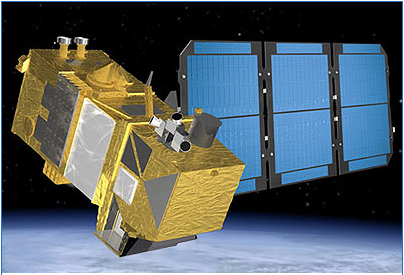
\includegraphics[width=250pt]{SENTINEL2AINTER.PNG}
  \caption{Satelitul Sentinel 2A \cite{sentinel2a}}   
\end{figure}

\subsubsection{Sentinel 2A benzi spectrale}

Benzile Sentinel 2A sunt imagini de tip TIFF cu o rezoluție între 7000 și 8000 pixeli,
cu 1 pixel reprezentând 10 de metri. O scenă acoperă aproximativ 290 km și este actualizată la
la fiecare 5 zile. Adâncimea de biți a imaginilor este de 12 . Pentru această lucrare am luat în considerare doar benzile trei(GREEN) și opt(NIR), întrucât acestea o să ne ajute la calcul indicelui de apa.

\subsubsection{Banda spectrală GREEN și NIR}

Banda spectrală GREEN este o culoare tradițională, întrucât face parte din grupul rgb(red,green,blue)și face partea din 'Natural Color Image'. Cu aceste benzi sunt generate imagini care au aspectul cel mai apropiat de o imagine reală.

Banda spectrală NIR măsoară infraroșu apropiat. Această parte a spectrului este deosebit de importantă pentru ecologie, deoarece plantele sănătoase o reflectă - apa din frunzele lor împrăștie lungimile de undă înapoi în cer. În comparație cu alte benzi, obținem indici precum NDWI, care ne permit să măsurăm sănătatea plantelor \cite{green}.


\begin{table}[ht]
\caption{Benzile spectrale NIR si GREEN \cite{nir}} % title of Table
\centering % used for centering table
\begin{tabular}{c c c c} % centered columns (4 columns)
\hline\hline %inserts double horizontal lines
 & Wave-lenght & Spatial Rezolution & Depth\\ [0.5ex] % inserts table
%heading
\hline % inserts single horizontal line
GREEN& 559 nm & 10 & 12 bit \\ % inserting body of the table
NIR & 832.9 nm & 10 & 12 bit\\
\hline %inserts single line
\end{tabular}
\label{table:nonlin} % is used to refer this table in the text
\end{table}


\subsubsection{Normalized difference water index}

Indicele de apă cu diferență normalizată (NDWI) se poate referi la unul dintre cel puțin doi indici derivați de teledetecție legați de apa lichida. Unul dintre acești indici este folosit pentru a măsură cantitatea de apa din frunzele platelor ,iar celelalt este folosit pentru a monitoriza schimbările care sunt aduse râurilor,lacurilor etc \cite{ndwi}.


 Formula pentru NDWI conține doua benzi importante :NIR (near-infrared) și  RED\cite{ndwi}:
    $$ NDWI = \frac{GREEN-NIR}{GREEN+NIR} $$
    
    Pentru a putea interpreta acesta formula și pentru evita crearea de alarme false se folosesc doua valori[20]:
   
       $<$ 0.3 - non-apă
       
    $>$ = 0.3 - apă
    
 \subsection{Limbajul de programare Python}
 
 Python este un limbaj de programare dinamic multi-paradigmă, creat în anul 1989 de programatorul olandez Guido van Rossum.. Structurile sale de date încorporate la nivel înalt, combinate cu tastarea dinamică, îl fac foarte atractiv pentru dezvoltarea rapidă a aplicațiilor, precum și pentru utilizarea ca limbaj de scrierea anumitor scripturi \cite{python}.
 
Python acceptă module și pachete, ceea ce încurajează modularitatea programului și reutilizarea codului. Interpretul Python și biblioteca standard extinsă sunt disponibile sub formă sursă sau binară fără taxe pentru toate platformele majore și pot fi distribuite în mod liber \cite{python}.

Limbajul de programare Python acordă  acces la mai multe biblioteci open-source care pot să fie ca un puzzle pentru a crea o anumită aplicație. Datorită flexibilității și simplității sale, Python a fost ales ca limbaj de baza în crearea acestui script pentru aplicația Qgis. 

\subsection{Pycharm}

Partea aplicativă a fost scrisă în PyCharm IDE, care este specializat în limbajul de programare Python. IDE asigură scrierea codului curat prin analizarea acestuia și suportă controlul reviziei cu sisteme precum Git, care a fost utilizat pentru controlul versiunii de scriere a aplicației. IDE este o  multiplataforma pe Windows, Mac OS și Linux.\cite{py} Am ales Pycharm  pentru dezvoltarea aplicației, deoarece include caracteristici precum asistența codului, re-factoring și controlul revizuirii cu Git \cite{py}.

\newpage
\section*{\bf Capitolul 3}
\markright{}
\section*{{\bf Tehnologii }}
\markright{}
\addcontentsline{toc}{section}{Tehnologii}
\setcounter{section}{1}
\refstepcounter{section}{}
\subsection{Quantum Gis}
\subsubsection{Despre Quantum GIS}
Gis (Geographic Information System) este o aplicație pentru sistemele geografice internaționale open source. Aceasta poate fi descărcată pe desktop.GIS permite utilizatorilor să editeze și să analizeze datele georgrafice, dar și să importeze și exporteze datele pe care aceștia le-au prelucrat.Aplicația Qgis oferă și varianta de a putea deschide harți digitale de pe computer, întrucât acestea suporta și adăugarea de noi informații, dar și tipărirea acestora.Aplicația are atât date de tip raster și, cât și date vectoriale. Datele vectoriale sunt stocate fie ca puncte, lini sau poligone. GIS este o aplicație care ajută la georeferențierea harților. Aplicația are și o multitudine de scripuri care ajută utilizatorul să facă cât mai multe îmbunătățiri și evidențieri pe care acesta dorește să le aplice \cite{qgis2}. Scripturile sunt scrise în limbajele de progrmare python și c++. O alta parte interesantă a acestui tool este acela că este, intradevar, o aplicație complexa. Câteva din funcțiile pe care GIS le are sunt: geocod(geocode), acesta este folosit pentru a crea puncte pe o hartă din adrese stradale sub forma de foaie de calcul, suprapunerea(overay), pentru a suprapune două sau mai multe harți sau straturi în același sistem de coordonate, pentru a arăta relațiile și a scoate în evidență diferențele  dintre ele, georeferența(georeference), pentru a alinia datele geografice (harta, strat) cu un sistem de coordonate dat, permițând suprapuneri si  buffer, pentru a crea o zonă în jurul unei caracteristici în unități de distantă sau de timp \cite{qgis}.
\subsection{QT Creator}
\subsubsection{Despre QT}
Qt Creator este un IDE pe mai multe platforme (Windows, Linux, Mac) care face parte din Qt SDK și are ca scop simplificarea dezvoltării aplicațiilor GUI pe mai multe platforme. Acest IDE este potrivit pentru dezvoltatorii care doresc să creeze aplicații pentru dispozitive incorporate, desktop.Am optat pentru a dezvolta un plugin în GIS cu acesta IDE, întrucât chiar aplicația GIS este scrisă folosind Qt.Astfel pentru dezvoltarea pluginului, am folosit aplicație Qt creator, pentru a putea proiecta interfață \cite{qt}.


\subsection{Scripturi python}
Deoarece limbajul de programare pe care îl folosim este python, trebuie să instalam legăturile acestui limbaj pentru Qt.În cazul în care s-a descărcat pachetul OSGEo4w în alt fișier o să schimbam acel path cu path-ul nostru. Că și instrument pentru linia de comanda vom folosi pyrcc5. La început am creat un fișier Windows Batch(.bat). Conținutul acestui fișier a fost următorul \cite{script} :



\begin{figure}[H]
  \centering
  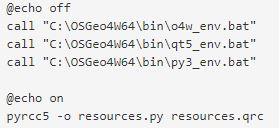
\includegraphics[width=250pt]{Capture.JPG}
  \caption{Executabil \cite{script}}   
\end{figure}

Ulterior vom copia acest fișier în folderul plugin.

\subsubsection{Rularea scripturilor în Quantum Gis}

Pentru a putea rula scripturi ân Qgis ne vom folosi de funcția pe care o are Qgis numită plugin builder.


\begin{figure}[H]
  \centering
  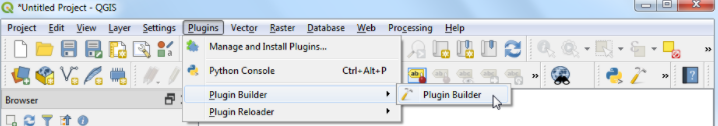
\includegraphics[width=300pt]{qgispluginPNG.PNG}
  \caption{Creare plugin  în Qgis \cite{script}}   
\end{figure}

Pentru a putea să beneficiem de acest plugin, trebuie ca acesta să fie instalat din Plugins - Manage and Install Plugins.

Dupa ce completam toate câmpurile și alegem folderul în care dorim ca plugin-ul a fie alocat  trebuie să ne apară casuța urmatoare :

\begin{figure}[H]
  \centering
  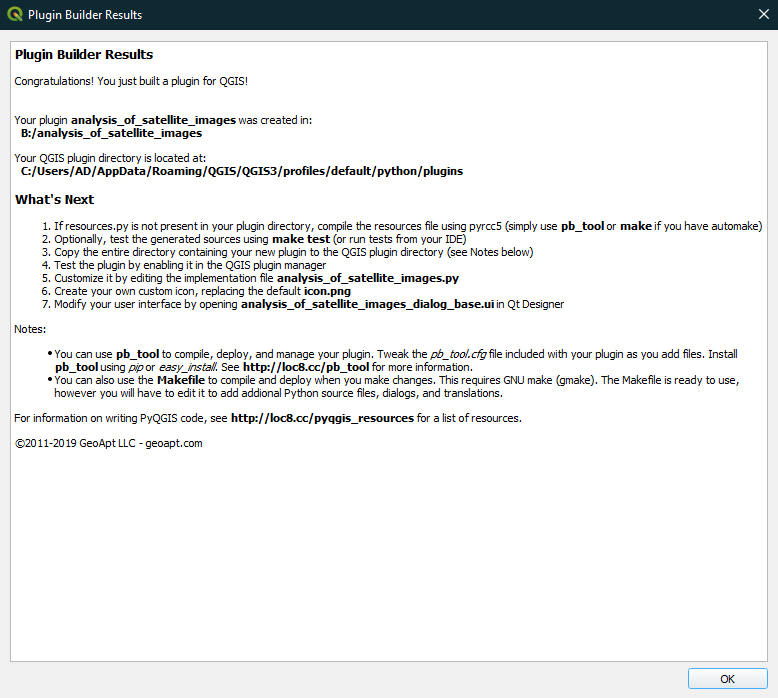
\includegraphics[width=300pt]{saveplugin.PNG}
  \caption{Crearea cu succes a pluginului în Qgis }   
\end{figure}

Acesta ne va asigura că am putut să generam plugin-ul în Qgis cu succes. Executabilul care contine path-urile (.bat) va trebuie să îl copiem in fișierul cu plugin-ul nostru. După rularea acestuia trebuie să ne apara două fisiere importante :


\begin{figure}[H]
  \centering
  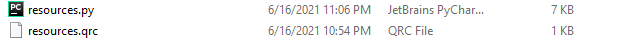
\includegraphics[width=300pt]{fisierePNG.PNG}
  \caption{Fișiere .py si .qrc}   
\end{figure}

După generarea celor 2 fișiere, că să putem folosi pluginul în aplicația Qgis va trebuie să merge în partea de sus a aplicație Qgis, selectăm settings - ușer profiles - open profile folder, de unde ne alegem fișierul cu plugin-ul. 


\begin{figure}[H]
  \centering
  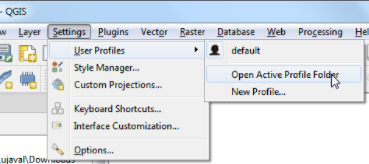
\includegraphics[width=300pt]{addplugin.PNG}
  \caption{Adăugarea pluginului în Qgis \cite{script}}   
\end{figure}

După ce instalăm acest plugin, va trebuie să îl adaugăm și în aplicația QtCreator, pentru a putea dezvolta interfață pentru plugin. Fișierele generate de către Qgis se salvează în AppData, iar de acolo trebuie să încarcăm folderul în QtCreator pentru a se putea salva modificările aduse.




\subsubsection{Biblioteci folosite}

În ultimul timp sunt folosite foarte mult date spațiale ,mai ales datele transmise prin satelit. Toate aceste date se află în biblioteca Earth Engine. Aceasta include o varietate de seturi de date pentru a putea oberva Pământul și schimbările acestuia. Earth Engine include : SRTM care are ca și rezoluție 30 m,
OpenLandMap care este un  set de date care conține proprietațiile solului și, de asemenea acesta are ca și rezoluție 250 m și GRIDMET care conține date depre temperatura și precipitați \cite{ee}.

Datele pe care acesta le conține sunt de mai multe categori: Features, Images and Collections. Pentru acest plugin am folosit datele de tip collections, întrucât aceste sunt o combinație între datele de tip features (ee.FeatureCollectionn)si  image(ee.ImageCollection) \cite{ee}.

\begin{figure}[H]
  \centering
  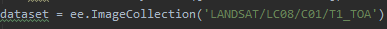
\includegraphics[width=300pt]{landsat.PNG}
  \caption{Importarea de imagini satelitare din satelitul Landsat}   
\end{figure}

Pentru NDVI (normalized difference vegetation index) am optat pentru a prelua imagini satelitare din satelitul Landsat8. Acesta conține unsprezece benci spectrale. Doua dintre acestea find folosite pentru a putea genera NDVI.

\begin{figure}[H]
  \centering
  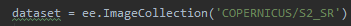
\includegraphics[width=300pt]{sentinel.PNG}
  \caption{Importarea de imagii satelitare din satelitul Sentinel 2A}   
\end{figure}

Pentru NDWI(normalized Difference Water Index ) am ales satelitul SENTINEL 2A de unde vom prelua imaginile, deoarece acesta are o rezolutie spațială speacială pentru cele doua benzi pe care le vom folosi. Rezoluția spațială pentru cele doua benzi find de 10 m.

\newpage
\section*{\bf Capitolul 4}
\markright{}
\section*{{\bf Arhitectura aplica\c tiei}}
\markright{}
\addcontentsline{toc}{section}{Arhitectura Aplicatiei}
\setcounter{section}{1}
\refstepcounter{section}{}
\subsection{Descrierea arhitecturi}

   Licență constă într-un plugin conceput special pentru aplicația Qgis. Astfel că codul principal a fost generat folosind un plugin al programului Qgis numit plugin builder. Acesta generează o structură de foldere și fișiere în mod automat care conțin fișiere atât de tip .py în care se afla functionalitatiile pluginului, cât și fișiere .xml care se ocupă de partea vizuală. Pentru  prelucrarea mai ușoară a părți vizuale s-a folosit aplicația Qt Creator care facilitează crearea unui design al interfeței fară a fi necesare modificări în structura de cod. 
    
    Pentru a da funcționalitate butoanelor din interfață am scris codul în limbajul de programare python în fișierul principal al structuri (analysis of satellite images dialog.py)
    
    În fișierul principal toate functionaliățtile pe care le-am implementat pentru plugin sunt împărțite în funcții cu sau fară parametri pe care le apelăm la momentul realizări unei acțiuni. Conexiunea între funcțiile definite și interfață propriu-zisă se realiază în interiorul funcției init(). Pentru fiecare element de interfață căruia vrem să îi atribuim o acțiune definită de noi îi adaugăm un lisener care în momentul în care se acționează, să apeleze o funcție specificată de noi.
    

\begin{figure}[H]
  \centering
  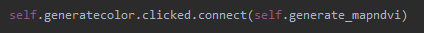
\includegraphics[width=300pt]{click.PNG}
  \caption{Apelare funcție la apăsarea unui buton}   
\end{figure}
  
  În figura 12 se poate vedea modul în care apelăm o funcție la apăsarea unui buton. Varibila generatecolor este o variabila generată automat de către Qt Creator la momentul adăugări unui buton în interfață, aceasta fiind legătură dintre partea de cod și partea vizuala. Pentru a-i da o funcționalitate, variabila find de tip QPushButton, aceasta conține funcție clicked() care funcționează pe post de listener și notifică butonul atunci când este apăsat din interfață. Pentru a îndeplini o acțiune la apăsarea butonului listenerului îi vom adaugă o conexiune la funcția noastră, modul în care realiazăm aceasta conexiune e prin apelarea funcției connect(). Atfel la fiecare apasarea a butonului se va apela funcția definita de către noi.

\subsection{Diagrama de stări}

\begin{figure}[H]
  \centering
  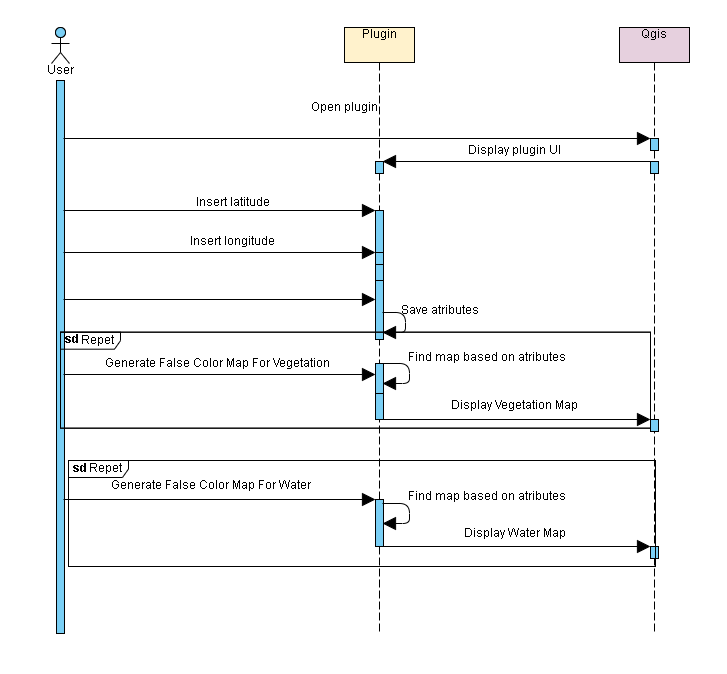
\includegraphics[width=300pt]{diagramastariPNG.PNG}
  \caption{Diagrama de stări}   
\end{figure}



\subsection{Funcționalitățile aplica\c tiei}

Utilizatorul odată intrat în aplicația va avea posibilitatea de a alege o locație anume din care dorește să genereze imaginile satelitare.Selectarea locației se face prin completare celor 2 câmpuri destinate acestei acțiuni (câmpul de latitudine și longitudine). În aceste câmpuri se vor completa coordonatele aferente locației în format de grade decimale. Dacă aceste câmpuri nu vor fi completate imagea se va genera folosind valorile default. Pentru această acțiunea am avut nevoie de pachetul EARTH Engine care face legătură cu baza de date a satelitul. Pentru NDVI am folosit satelitul Landsat 8, iar pentru NDWI am folosit satelitul Sentinel 2A. 

Când extragem aceste imagini satelitare, le extragem sub formă de listă. Pentru a putea genera o singură imagine satelitare, lista pe care am extras-o din baza de date a satelitului trebuie să indeplineasă anumite caracteristici, cum ar fi acoperirea de norilor. Am filtrat aceste poze după o acoperiră minima, întrucât dorim ca atunci când ne generăm imaginea aceasta să fie cât mai clara.

Cu funcția default first(), algortimul ne va retuna prima poza din lista care se încadrează cel mai bine în caracteristile date.


În continuare pe lângă coordonate, utilizatorul are posibilitatea de a-și alege momentul în care dorește să se genereze imaginea satelitara. Pentru această acțiune, exita două butoane de tipul QdateEdit.Aceste butoane setează ziua, luna și anul în care se dorește a  genera imaginea satelitara. Funcționalitate pe care acestea o au este de a seta un interval de timp în care satelitul a  realizat o imagine în coordonate și intrevalul setat de către utilizator.

Butonul 'Generate Flase Color Map for Vegetation' ne generază o hartă cu ajutorul benzilor spectrale. Pentru aceasta functionaliate ne-am ajutat de formula pentru NDVI care folosește două benzi (red și nir). La apăsarea butonului utilizatorul va putea observa harta generată .

Butonul 'Generate Flase Color Map for Water' ne generază o harta cu ajutorul benzilor spectrale. Pentru acestea functionaliate ne-am ajutat de formula pentru NDWI care folosește două benzi (green și nir). La apăsarea butonului utilizatorul va putea observa harta generată.

În funcție de intervalul pe care utlizatorul îl alege plugin-ul o să genereze câte o imagine din fiecare an, atât timp cât exista imagini în baza de date a satelitului. De asemenea plugin-ul va selecta și cea mai bună imagine din acel an, astfel ca în final acesta va genera cea mai bună harta din acel an.După generarea imaginilor acesta poate să aleagă doi ani dintre cei generați pentru a putea vedea procentual diferență dintre cele doua harți.

Am realizat și un buton 'Reset' care ne resetează coordonatele ,timpul si butoanele ca să poate fi din nou active.


\subsection{Interfa\c ta aplica\c tiei}


Interfața pluginului este una minimalistă și în același timp ușor de înțeles. Utilizatorul trebuie doar să intaleze scriptul din bara de sus a aplicația Qgis.

\begin{figure}[H]
  \centering
  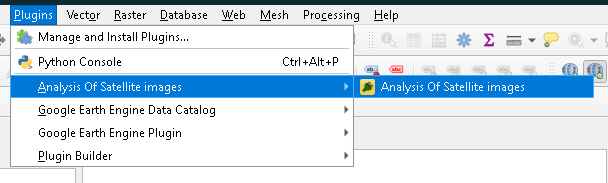
\includegraphics[width=250pt]{analiza.PNG}
  \caption{Instalare plugin în Qgis}   
\end{figure}



\begin{figure}[H]
  \centering
  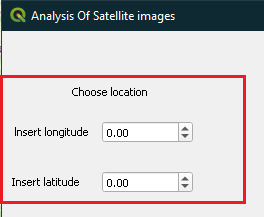
\includegraphics[width=250pt]{location.PNG}
  \caption{Alegerea coordonatelor}   
\end{figure}

După aceea utilizatorul trebuie să insereze coordonatele pe care acesta le dorește. Pentru butonul 'Insert latitude' acesta va inserva latitudinea, iar pentru butonul 'Insert longitude' va insera longitudinea. Completarea coordonatelor unde acesta dorește să genereze harta vor trebuie să fie de tip decimal. 

Daca utilizatorul nu va completa aceste două câmpuri scriptul va genera o hartă cu coordonatele sale default.

\begin{figure}[H]
  \centering
  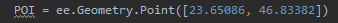
\includegraphics[width=300pt]{coordonate defalut.PNG}
  \caption{Coordonatele default ale pluginului}   
\end{figure}

După alegerea coordonatelor, utilizatorul trebuie să își aleagă intervalul în care dorește să îi se genereze harta. Pentru această acțiune aveam două butoane. Cele două butone vor prelua toate datele introduse de către utilizator anterior și folosindu-se de datele respective vor caută imagini satelitare corespunzătoare cu cerințele utilizatorului și vor performa anumite modificări asupra lor.Dacă pluginul avea doar un singur buton acesta putea să duca la o eroare, deoarece satelitul nu realizează în orice moment al zile imaini satelitare în anumite coordonate specifice. 


\begin{figure}[H]
  \centering
  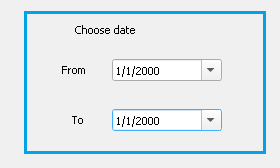
\includegraphics[width=250pt]{date.PNG}
  \caption{Alegerea intervalului de timp}   
\end{figure}

După ce utilizatorul introduce toate datele dorite pentru a-și putea realiza o hartă, acesta poate genera o mapă pentru a putea observa schimbările pentru vegetație(păduri) și pentru apa (râuri, lacuri). La apăsarea butonului 'Generate False Color Map for Vegetation' algoritmul va genera mai multe hărti în funcție de intervalul pe care l-a alocat utilizatorul.

\begin{figure}[H]
  \centering
  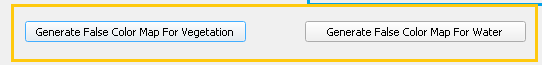
\includegraphics[width=300pt]{butoanenoi.PNG}
  \caption{Generarea hărților}   
\end{figure}



Hărțile  care vor fi generate vor fi de forma NDVI, unde vom putea observa accentuarea zonelor de vegetație.
În aceaste poze putem observa că ceea ce înainte a fost zona de vegetație acum este evidențiată cu roșu aprins. Acest lucru se datorează benzi spectrale NIR. Întrucât conform caracteristicilor spectrale ale vegetației, plantele stufoase au o reflectanță redusă asupra benzi roșii, dar acestea au arătat o corelație ridicată cu ,LDBM(leaf dry bomass matter) și conținutul de clorofilă al frunzelor \cite{leaf2}. Din cauza clorofile prezente în frunze ,răspunsul spectral pe care acestea o sa ni-l dea  este unul foarte ridicat. Acest răspuns este intens în NIR, dar aproape invizibil în alte porțiuni \cite{leaf}.


Dacă utilizatorul dorește să genereze celalalt tip de hartă, acesta doar trebuie să apese butonul 'Reset' iar el va putea să introducă aceleași date sau date diferite,intervale de tip diferite pentru a  putea genera o imagine nouă.  La apăsarea butonului 'Generate False Color Map for Water' algoritmul va genera mai multe hărti în funcție de intervalul pe care l-a alocat utilizatorul.


Celelalte hărți care vor fi generate vor fi de forma NDVI, unde vom putea observa accentuarea zonelor unde există corpuri de apa(râuri și lacuri).

După ce plugin-ul a generat hărțile, utilizatorul trebuie să aleagă ani în care dorește să vadă diferență, mai precis schimbările care s-au produs în decurs de un an. Acest lucru îl va face cu ajutorul celor doua butoane de tip drop down, de unde poate să își aleagă ani care sunt valabili pentru imaginile generate în intervalul alocat de el.

\begin{figure}[H]
  \centering
  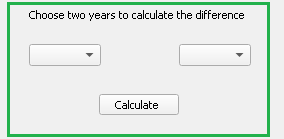
\includegraphics[width=250pt]{drop down.PNG}
  \caption{Alegerea hărților }   
\end{figure}

După apăsarea butonului 'Calculate', această va calcula diferență de pixeli dintre cei doi ani aleși de către utilizator.
La apăsarea butonului 'Cancel' plugin-ul se va închide, iar după aceea puteam să îl deschidem din nou. 
 
\newpage 
\section*{\bf Capitolul 5}
\markright{}
\section*{{\bf Detalii de implementare}}
\addcontentsline{toc}{section}{Detalii de implementare}
\setcounter{section}{3}
\subsection{Realizarea interfe\c tei}

Interfața am realizat-o în aplicația Qt Creator. Această aplicație este de tipul drag and drop și ,de aemenea, dispune și de anumite butoane speciale pentru alcătuirea unei interfețe.



\begin{figure}[H]
  \centering
  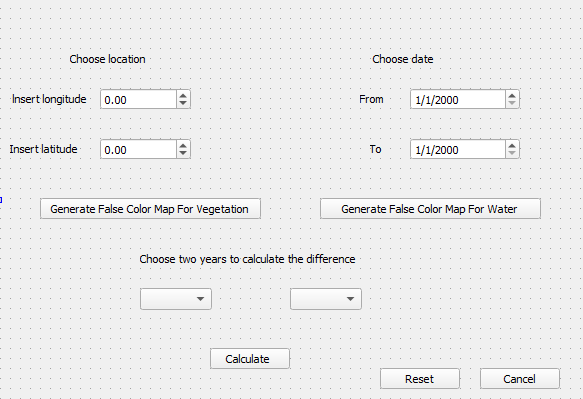
\includegraphics[width=300pt]{guinou.png}
  \caption{Interfața în aplicația Qt Creator}   
\end{figure}


Pentru label-urile 'Choose location', 'Choose date  'Insert latitude','Insert longitude', 'From', 'To'și 'Choose two years to calculate the difference' am folosit label-urile de tip QLabel. QLabel este utilizat pentru afișarea textului sau a unei imagini. Nu este furnizată nicio funcționalitate de interacțiune cu utilizatorul. Aspectul vizual al etichetei poate fi configurat în diferite moduri.

Pentru câmpurile unde putem insera coodonatele dorite, am folosit două butoane de tipul QDoubleSpinBox.
QDoubleSpinBox permite utilizatorului să aleagă o valoare făcând clic pe butoanele sus sau jos sau apăsând sus sau jos de pe tastatură pentru a mări sau micșora valoarea afișată în prezent. De asemenea, utilizatorul poate introduce manual valoarea. Caseta de rotire acceptă valori double, dar poate fi extinsă pentru a utiliza șiruri diferite cum ar fi: textFromValue () și valueFromText () \cite{coordonate}.

Butoanele care ne ajuta să setam intervalul de timp sunt de tipul QDateEdit.

QDateTimeEdit permite utilizatorului să modifice datele folosind tastatura sau tastele săgeată pentru a mări și micșora valorile datei și orei. Tastele săgeți pot fi folosite pentru a va deplasa de la secțiune la o alta  secțiune din caseta QDateTimeEdit. Datele și orele apar în conformitate cu formatul stabilit \cite{date}.

Gama de valori valide pentru un QDateTimeEdit este controlată de proprietățile minimumDateTime, maximumDateTime și componentele respective de dată și oră. În mod implicit, orice dată-oră de la începutul anului 100 CE până la sfârșitul anului 9999 CE este validă \cite{date}.

Iar butoanele 'Generate False Color Map For Vegetation' , 'Generate False Color Map For Water', 'Calculate', 'Reset' si 'Cancel' sunt de tip QPushButton.

QPushButton este probabil cel mai frecvent widget utilizat în orice interfață grafică de utilizator. Apăsați pe un buton pentru a comanda computerului să efectueze o acțiune sau pentru a răspunde la o întrebare. 
QPushButton este dreptunghiular și de obicei afișează o etichetă text care descrie acțiunea acestuia.\cite{generare}

Pentru cele două butoane de unde puteam alege ani între care dorim să se afișeze diferențele dintre cele două harți pe care o să le generăm sunt de timpul comboBox.

ComboBox este un widget de selecție care afișează elementul curent șipoate afișa o listă de elemente selectabile. Un buton de tipul comboBox poate fi editabil, permițând utilizatorului să modifice fiecare articol din listă \cite{combo}.

\subsection{Formule pentru prelucarea benzilor}
Pentru putea evidenția mai ușor imaginile satelitare am folosit două formule specifice pentru NDVI (Normalized Difference Vegetation Index) și pentru NDWI(Normalized difference water index).
    Formula pentru NDVI conține două benzi importante :NIR (near-infrared) și  RED:
    $$ NDVI = \frac{NIR-RED}{NIR+RED} $$
   În python aceasta se scrie în următorul mod:
    \begin{figure}[H]
  \centering
  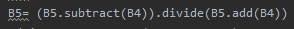
\includegraphics[width=300pt]{ndvi.PNG}
  \caption{NDVI formula}   
\end{figure}

    ,unde funcția .substract scade a doua valoare din prima pentru fiecare pereche de benzi potrivite din imaginea1 și imaginea2. Dacă image1 sau image2 are doar o bandă, atunci este utilizată împotriva tuturor benzilor din cealaltă imagine. Funcția .divide este împărțirea celor doua ecuații, iar funcția .add adaugă prima valoare la a doua pentru fiecare pereche de benzi potrivite din imaginea 1 și imaginea 2. Dacă image 1 sau image 2 are doar o bandă, atunci este utilizată împotrivă tuturor benzilor din cealaltă imagine \cite{formula}.
    
     Formula pentru NDWI conține și ea două benzi importante : GREEN și NIR (near-infrared):
    $$ NDWI = \frac{GREEN-NIR}{GREEN+NIR} $$
   
  În python aceasta se scrie în următorul mod:
\begin{figure}[H]
  \centering
  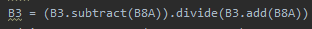
\includegraphics[width=300pt]{ndwi.PNG}
  \caption{NDWI formula}   
\end{figure}

    
     ,unde funcția .substract scade a doua valoare din prima pentru fiecare pereche de benzi potrivite din imaginea1 și imaginea2. Dacă image1 sau image2 are doar o bandă, atunci este utilizată împotriva tuturor benzilor din cealaltă imagine. Funcția .divide este împărțirea celor doua ecuații, iar funcția .add adaugă prima valoare la a doua pentru fiecare pereche de benzi potrivite din imaginea 1 și imaginea 2. Dacă image 1 sau image 2 are doar o bandă, atunci este utilizată împotrivă tuturor benzilor din cealaltă
     imagine \cite{formula}.
\subsubsection{Rezultatele prelucări benzilor spectrale}

La apăsare butonului 'Generate False Color Map for Vegetation', s-au generat mai multe  hărti care surprind schimbările aduse pe parcursul anilor asupra pădurilor.

\begin{figure}[H]
  \centering
  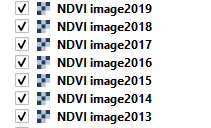
\includegraphics[width=250pt]{ani.PNG}
  \caption{Generarea hărților in intervalul de timp 2000-2020}   
\end{figure}

Cum putem observa și în figura 23, pentru intervalul de timp alocat 2000-2020 sau generat șapte hărti. Aceste hărti fiind prelucrare cu ajutorul formulei pentru NDVI.

Dintre acestea am ales ceLE mai semnificativE pentru a o putea analiza.

\begin{figure}[!htb]
   \begin{minipage}{0.48\textwidth}
     \centering
     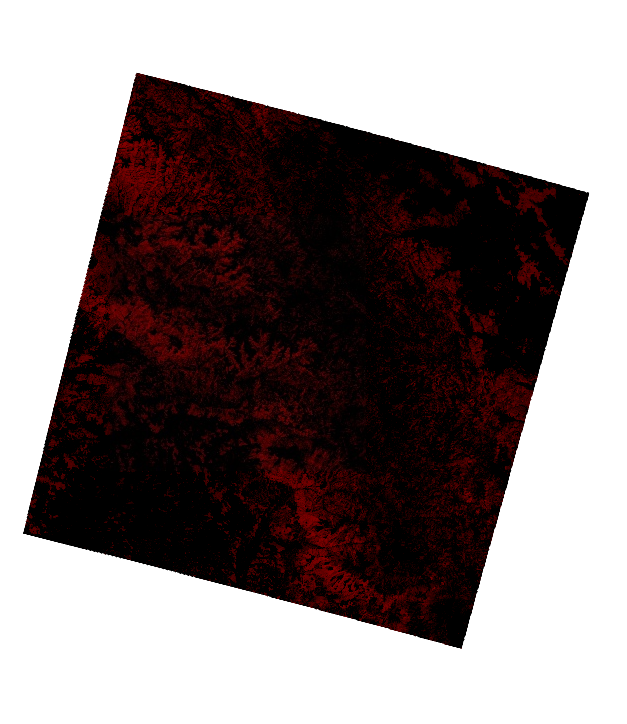
\includegraphics[width=1\linewidth]{ndvinou3.png}
     \caption{NDVI 2015}
   \end{minipage}\hfill
   \begin{minipage}{0.48\textwidth}
     \centering
     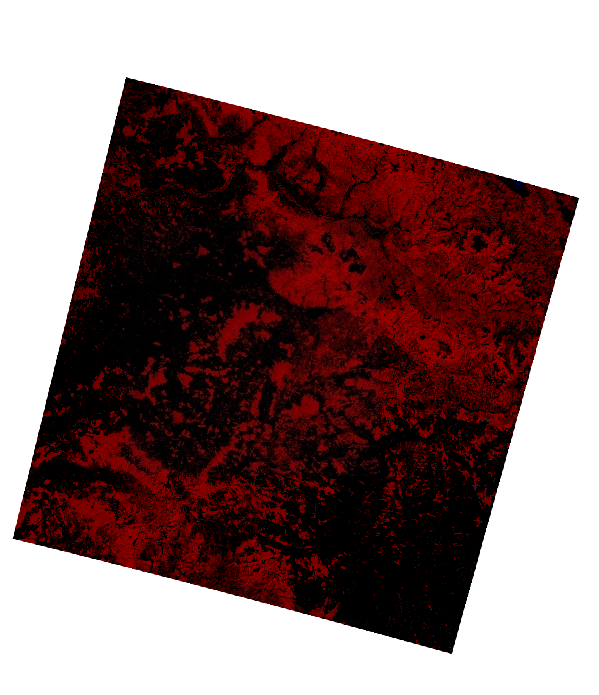
\includegraphics[width=1\linewidth]{ndvinou.png}
     \caption{NDVI 2017}
   \end{minipage}
\end{figure}
Datorită clorofile care se găsește în plantele verzi și a bandei spectrale NIR, putem oberva cu ușurință că pădure este evidențiată cu un roșu puternic, astfel făcând-o mult mai ușor vizibilă în cadrul imagini. Iar ceea ce este împrejurul pădurii find evidențiat  cu negru , acest lucru făcând posibil evidențierea și mai tare a păduri.

La apăsare butonului 'Generate False Color Map for Water', s-au generat mai multe  hărti care surprind schimbările aduse pe parcursul anilor asupra râurilor și lacurilor.


\begin{figure}[H]
  \centering
  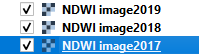
\includegraphics[width=250pt]{hartinoi.PNG}
  \caption{Generarea hărților in intervalul de timp 2000-2020}   
\end{figure}

Cum putem observa și în figura 26, pentru intervalul de timp alocat 2000-2020 sau generat trei hărti. Aceste hărti fiind prelucrare cu ajutorul formulei pentru NDWI.

Dintre acestea am ales cea mai semnificativă pentru a o putea analiza.


\begin{figure}[!htb]
   \begin{minipage}{0.48\textwidth}
     \centering
     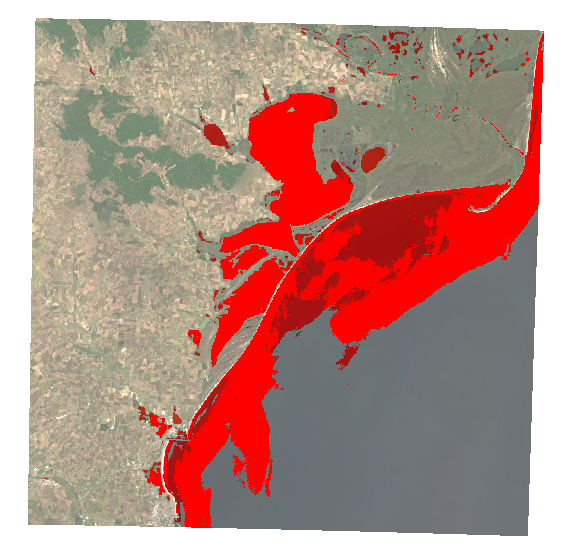
\includegraphics[width=1\linewidth]{ndwinou2.PNG}
     \caption{NDWI 2018}
   \end{minipage}\hfill
   \begin{minipage}{0.48\textwidth}
     \centering
     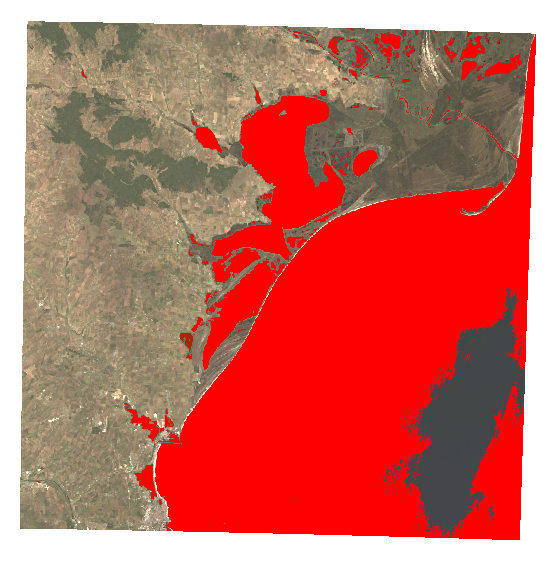
\includegraphics[width=1\linewidth]{ndwinou.PNG}
     \caption{NDWI 2019}
   \end{minipage}
\end{figure}
Datorită banzi  spectrale NIR, putem oberva cu ușurință că apa este evidențiată cu un roșu puternic, astfel făcând-o mult mai ușor vizibilă în cadrul imagini. Iar ceea ce este împrejurul apei find mascat și prelucrat cu ajutorul opacități, pentru a putea observa mai ușor corpurile de apă.



\subsection{Scripturi}
\subsubsection{Preluarea imaginilor}

Pentru preluarea imaginilor satelitare vom folosi funcții oferite de către biblioteca Earth Engine pentru a putea accesa bazele de date a anumitor sateliți.

\begin{figure}[H]
  \centering
  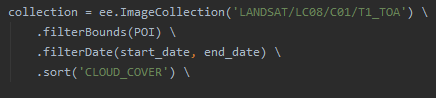
\includegraphics[width=300pt]{landsatsatelit.png}
  \caption{Preluare imgini satelitare}   
\end{figure}


\begin{figure}[H]
  \centering
  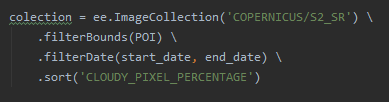
\includegraphics[width=300pt]{sentinelsatelit.png}
  \caption{Preluare imagini satelitare}   
\end{figure}

Pentru accesarea unei baze de date specifice vom apela funcția ee.ImageCollection() care ia că și parametru numele satelitului a cărui imagini dorim să le accesam. Aceasta functie returnează un vector de imagini pe care putem mai departe să-l fitram pentru a ajunge la imaginea dorită. 

Primul filtrul pe care îl aplicăm asupra vectorului este filterBounds care ia ca și parametru un obiect de tip ee.Geometry.Point care conține două valori corespunzătoare latitudini și longitudini scrise în format decimal.Putem observa că oferim ca și parametru variabila POI care este variabila în care salvăm coordonatele introduce se către utlizator în cadrul pluginului.

Următorul filtru pe care îl vom folosi este filterDate acesta va lua ca și parametru două valori de tipul QDateEdit și reprezintă intrevalul de timp în care trebuie să se încadreze realizare pozei pentru a putea fi considerată relevantă.De asemenea variabilele $start_date$ și $end_date$ reprezintă variabilele în care salvăm datele introduse de către utilizator.

După ce am filtrat vectorul pe baza criteriilor de mai sus folosim o funcție sort() pentru a ne sorta imaginile în funcție de procentul de acoperire a norilor,astfel încât prima poza din vector să aibă un procentaj de acoperire cât mai mic.

În urma preluări, filtrări și sortări acestora vom obține o colecție de imagini dintr-un an specificat, într-o anumită locație specificată și sortate în așa fel încât prima să fie cu gradul de acoperire a norilor cel mai scăzut. Înainte să trecem la partea de prelucrare a aceastora mai avem o posibila problema care ar putea apărea. În momentul actual nu știm cu certitudine daca în baza de date a sateliților s-a găsit sau nu cel puțin o imagine corespunzătoare cu cerințele noastre. Pentru a evita situația în care s-ar ajunge dacă am încerca să prelucrăm o lista goală de poze, s-a folosit un block de tip try except.

În blocul try din colecția de poze obținută indiferent dacă aceasta este populată sau goală vom folosi funcția first() pentru a ne extrage din aceasta prima imagine găsită și a o salva într-o variabila de tip image. De asemenea toate celelalte calcule pe care urmează să le facem imagini se vor afla în blocul try. 

Astfel încât în cazul în care o imagine este goala sau apar alte erori din diverse motive execuția algoritmului va decurge în mod normal în continuare fară a a afișa o anumită eroare. Astfel utilizatorul va facilita de functionalitatiile aplicației, ne find întrerupt de posibilele erori care ar putea apărea în mod normal.

În final după sortare și după filtrare vom obține un vector de imagini în care pe prima poziție se afla imaginea care se încadrează cel mai bine în căutările noastre,astfel că vom folosi funcția first() pentru a putea extrage imaginea respectivă, neavand nevoie de restul imaginilor din vector.Ca prin urmare variabila collection va fi de tip image și va reține cea mai potrivită imagine din baza de date pentru prelucrările viitoare.

\subsubsection{Prelucrarea imaginilor satelitare}

Datorită atmosferei noastre, vedem doar porțiuni specifice ale spectrului electromagnetic.

\begin{figure}[H]
  \centering
  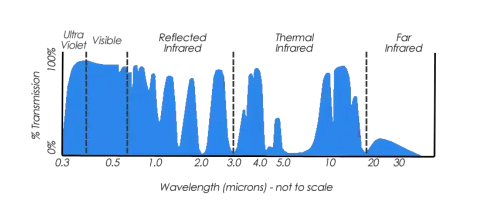
\includegraphics[width=400pt]{benzispectralePNG.PNG}
  \caption{Benzile spectrale \cite{benzi}}   
\end{figure}


Ochii noștri pot vedea doar porțiunea vizibilă - roșu, verde și albastru. Vegetația sănătoasă (sau clorofila) reflectă mai multă lumină verde comparativ cu alte lungimi de undă. Absoarbe mai multă lumină roșie și albastră. De aceea ochii noștri îl văd verde.\cite{benzi}

Dar anumite tipuri speciale de senzori pot prelua alte culori ale spectrului elctro magnetic invizibile pentru ochiul uman. De exemplu, vegetația reflectă și mai mult infraroșul(NIR). \cite{benzi}

Pentru a putea observa mai bine pădurile și apele o să ne ajutăm de două formule, formula pentru NDVI și formula pentru NDWI.

\begin{figure}[H]
  \centering
  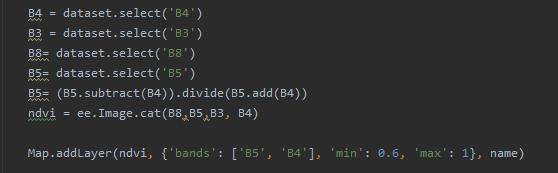
\includegraphics[width=300pt]{prelucrarebenzi.png}
  \caption{Prelucrarea imaginilor satelitare }   
\end{figure}

În variabila collection avem stocată imaginea obținută anterior în urma accesări bazei de date și a filtrări acesteia.În mod standard imaginile satelitare aflate în baza de date respectivă conțin un vector în care se ragăsesc toate tipurile de benzi. Pentru a realiza calculele dorite asupra imagini în scopul de a evidenția apa sau pădurile inițial va trebui să ne extragem din imaginea inițială benzile pe care dorim să le folosim mai departe în cadrul formulelor.



Acest lucru se realizează folosind funcția select() care va lua ca și parametru un string ce reprezintă numele benzi pe care dorim să o extragem. Aceasta funcție returnează un obiect de tip image dar care de această dată conține doar o singura bandă.Astfel că vom salva valoarea returnată de funcție într-o noua variabilă pe care o să o folosim mai departe la calcule.

Odată selectate benzile necesare putem să le înlocui în formula de calcul și vom obține o image care de asemenea conține o singură bandă, dar de această dată banda respectivă va evidenția elementul dorit. Având banda de evidențiere și câteva benzi standard dorim să ne  reconstruim pe baza acestora o nouă imagine care să conține toate benzile dorite printre care și cea folosită pentru calcul.


În final vom exporta către Qgis imaginea finală obtinută prin adăugarea acesteia într-un nou layer, acțiunea realizată de către funcția addLayer().

Generarerea diferențelor dintre două poze satelitare va folosi de asemenea o combinație a anumitor formule pentru a obține o filtrare corectă. De această dată formulele folosite nu vor mai fi de tip matematic, ci mai degrabă formule logice, folosindu-ne aici de rezultate obținute la pasi anteriori. 

Pentru început luând ca exemplu pădurile pentru determinarea zonelor defrișate vom selecta două imagini satelitare din ani diferiți cu pădurile evidențiate și vom căuta zonele împădurite care existau în prima imagine,dar nu se vor mai găsi în imaginea mai recentă.

Simultan pentru a descoperi zonele în care sau efectuat plantări vom aplica același proces doar că de această data în sens invers selectând toate zonele în care exista pădure în momentul actual, dar nu există într-un moment din trecut. Odată obținute rezultatele vom îmbina cele două hărti obținute într-o singura harta care va conține ,de asemenea un fundal format din imaginea orginala,dar setată la un grad de vizibilitatea mai mic, pentru a nu distrage atenția de la evidențieri.

\begin{figure}[H]
  \centering
  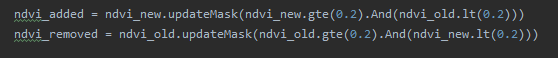
\includegraphics[width=300pt]{formuleevidentierindvi..PNG}
  \caption{Formule pentru evidențierea pădurilor }   
\end{figure}

\begin{figure}[H]
  \centering
  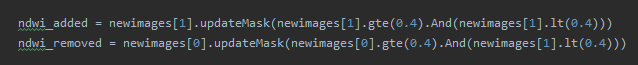
\includegraphics[width=300pt]{formule evidentierindwi.PNG}
  \caption{Formule pentru evidențierea apelor }   
\end{figure}


\subsubsection{Comparația imaginilor satelitare}
Odată generate toate imaginile satelitare următorul pas este oferirea unei utilități practice acestora. În contextul acestei lucrări vom exemplifica în mod automat diferențele dintre două perioade de timp surprinse cu ajutorul unei imagini satelitare cu scopul de a evidenția modificările săvârșite asupra acestora. Atât pentru cazul pădurilor, cât și pentru ape se urmărește evidențierea atât a evoluției acestora de la un an la altul, cât și a degradări acestora. 

În cazul pădurilor problema defrișărilor este una extrem de gravă pentru mediu.De asemenea având un nivel de gravitate similar este lipsa inițiativelor de replantare a pădurilor.Din acest motiv defrișând tot mai mult și plantând tot mai puțin în anumite zone suprafețele împădurite devin tot mai mici. 

În cadrul aplicației am reușit să realizăm într-un mod automat,din script atât evidențierea defrișărilor,cât și cea a plantări. Pentru a avea o vedere de ansamblu mai buna asupra acțiunilor ce se efectuează pădurilor.\newline

Exemplicarea funcționalități este mult mai ușoară în momentul în care facem referință la un exemplu concret.Pentru a vedea cât mai bine modul în care sunt afișate aceste două amănunte referitoare la păduri am ales să studiez zonele împădurite din Australia, într-o perioada obișinuită  în comparație cu datele satelitare obținute la începutul anului 2020.

În (figura 35) am ales aleatoriu doi ani pentru a ne procura datele referitoare la Împăduriri/despăduriri.în urma generări pozei putem observa că într-o perioadă normală în Australia gradul de despădurire este aproximativ echivalent, chiar mai mic decât gradul de împădurire. Acest lucru ne arată că în anumite zone a continentului în Australia apar noi păduri mult mai des, decât sunt tăiat cele vechi.

În schimb pentru a face o comparație cât mai vizibila și radicală am ales să iau ca și referință anul 2019, respectiv anul 2020.La începutul anului 2020 a avut loc unul dintre cele mai mari incendii din istoria continentului.Urmele devastării acestuia se pot observa clar, chiar și pe analiza satelitara realizată în cadrul acestei lucrări.În (figura 36) putem observa faptul că aproape întreagă imagine este acaparată de nuante  de roșu , reprezentând pierderi enorme de zone împădurite.
\begin{figure}[!htb]
   \begin{minipage}{0.48\textwidth}
     \centering
     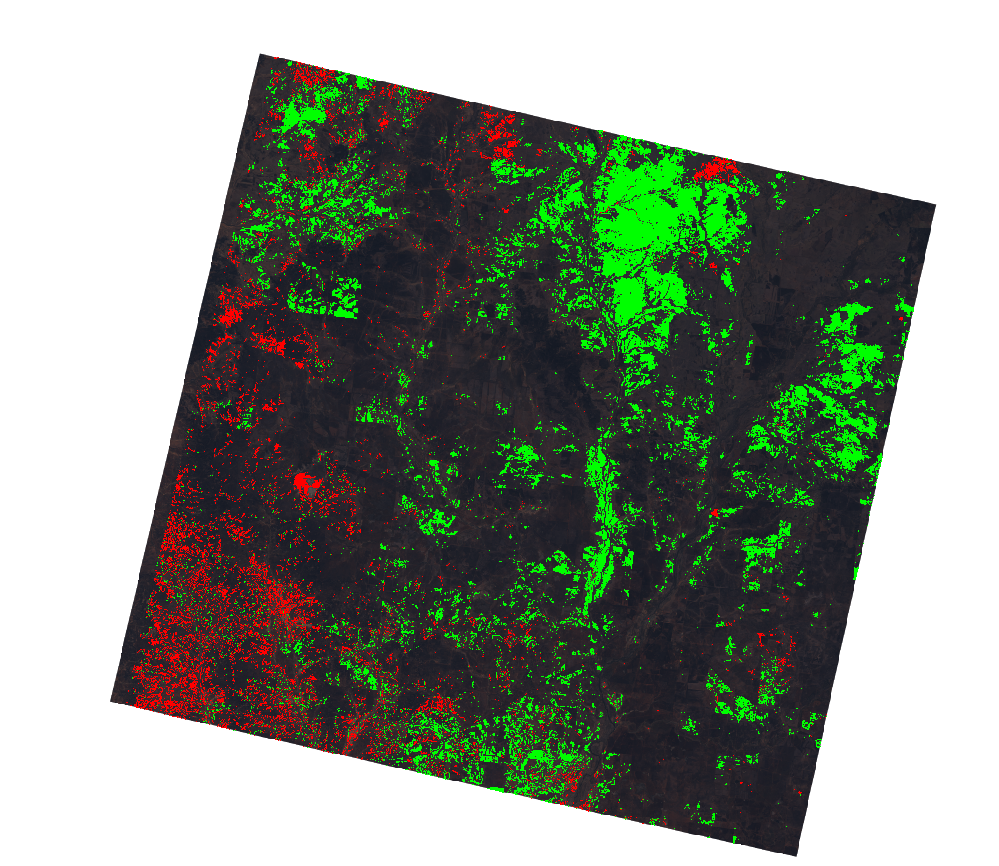
\includegraphics[width=1\linewidth]{ndvi2016-201.PNG}
     \caption{Analiza defrișări/impăduriri Australia 2016-2017}
   \end{minipage}\hfill
   \begin{minipage}{0.48\textwidth}
     \centering
     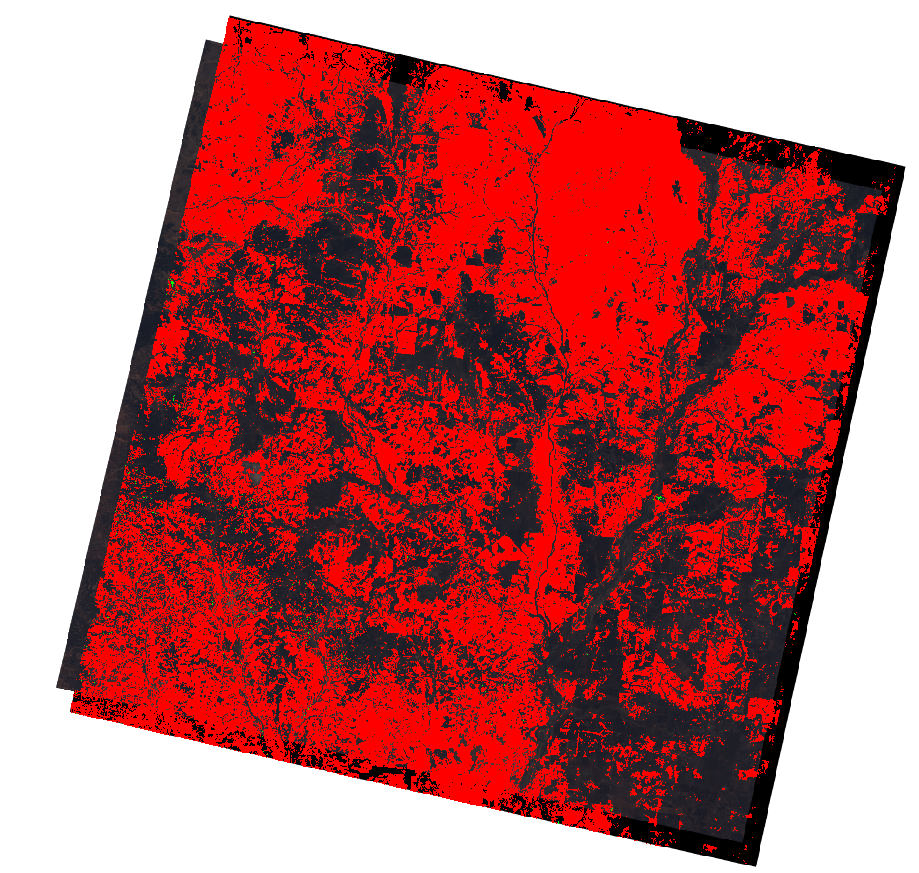
\includegraphics[width=1\linewidth]{ndvi2019-2020.PNG}
     \caption{Analiza defrișări/impăduriri Australia 2019-2020}
   \end{minipage}
\end{figure} 

\newpage
\subsubsection{Exportarea imaginilor satelitare}

Pentru a putea exporta imaginile satelitare  din aplicația Qgis, utilizatorul trebuie să facă acest lucru manual pentru a putea beneficia de hărțile prelucrate.Importat de reținut este faptul că nu trebuie salvată cu  ajutorul funcției SaveAs(),deoarece în momentul salvări acesta nu va fi o harta integrala.Utilizatorul trebuie  să meargă în meniul de sus al aplicația Qgis la Project și să selecteze Import/Export, de aici acestea are două opțiuni pentru a putea beneficia de aceste harți: 

\begin{figure}[H]
  \centering
  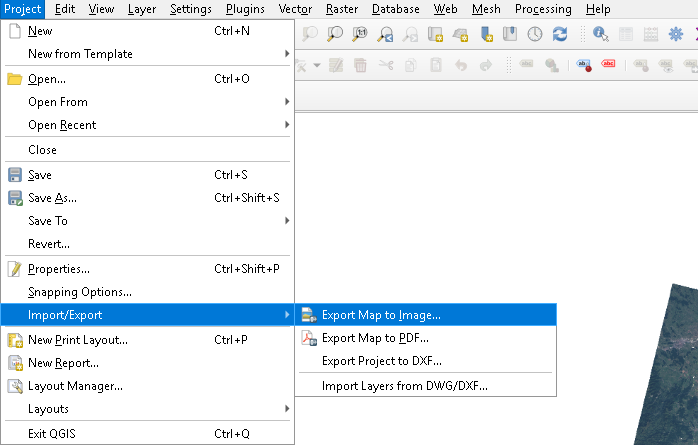
\includegraphics[width=250pt]{export image.PNG}
  \caption{Exportarea imaginlor din Qgis }   
\end{figure}

Prin această acțiunea utilizatorul va exporta harta în format .pqw.Deschirea acesteia se poate face doar cu un anumite IDE, întrucât acesta ne va returna doar anumite date despre hartă pe care noi am prelucrat-o.

Pentru a putea vizualiza harta aveam opțiunea să o salvăm în format .pdf. Acesta opțiune ne va genera harta într-un mod vizibil și cu o claritite destul bună.

\begin{figure}[H]
  \centering
  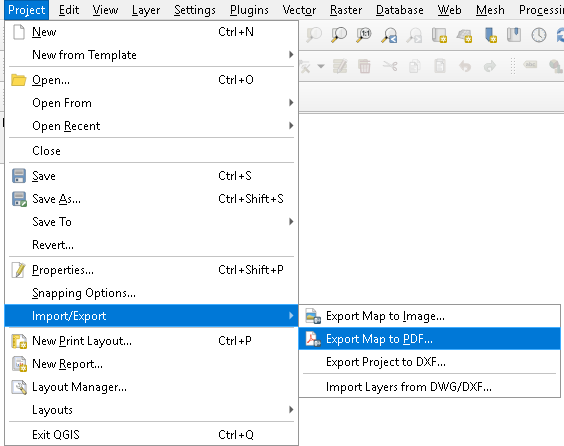
\includegraphics[width=250pt]{exportpdf.PNG}
  \caption{Exportarea imaginlor din Qgis }   
\end{figure}



\newpage
\section*{{\bf Concluzii}}
În concluzie observarea Pământului este foarte importanta și ,de semenea constă în numeroase cunoștinte. Scopul noasru a fost acela de a putea evidenția și concretiza schimbarea pădurilor și a apelor. Acest lucru făcând posibil ca toate informațiile să ajungă într-un mod mai rapid și mai eficient la oamenii de știință și persoanele responsabile.

Ceea ce se mai poate constata este că folosind anumite formule și prelucând benzile spectrale putem realiza anumite statistici și analize care pot aduce o schimbare asupra mediului.

Din alt punct de vedere, datele și imaginile generate ar putea fi utile pentru schimbările care se petrec în natura. Pădurile și apele având un rol important când vine vorba despre dezastre naturale.

\markright{}
\addcontentsline{toc}{section}{Concluzii}
\setcounter{section}{1}




\newpage
\begin{thebibliography}{9}
    \bibitem{wiki} 
    Satelitul Sputnik,
    \url{hhttps://en.wikipedia.org/wiki/Satellite}
    
    \bibitem{wikisputnik} 
    Satelitul Sentinel 2A,
    \url{https://eos.com/find-satellite/sentinel-2/}
    
    \bibitem{aplicati} 
    Aplicatii similare,
    \url{https://fsc.org/en/innovation/earth-observation}
    
    \bibitem{satelitare} 
   Imaginior Satelitare,
    \url{https://en.wikipedia.org/wiki/Timeline_of_first_images_of_Earth_from_space}
    
     \bibitem{istorie} 
   Scurta istorie a satelitilor,
    \url{https://atos.net/en/blog/a-brief-history-of-earth-observation}
    
    \bibitem{istorie2}
    \url{https://ec.europa.eu/jrc/en/research-topic/earth-observation}
    
         \bibitem{radiometrica} 
   Rezolutia radiometrice,
    \url{https://www.fis.uni-bonn.de/en/recherchetools/infobox/professionals/resolution}
    
       \bibitem{temporala} 
   Rezolutia temporale si spectrale,
    \url{https://sentinels.copernicus.eu/web/sentinel/missions/sentinel-2/instrument-payload/resolution-and-swath}
    
        \bibitem{spatiala} 
   Rezolutia spatiale,
    \url{atimagingcorp.com/satellite-sensors/other-satellite-sensors/landsat-8/}
    
       \bibitem{spatialasentinel} 
   Rezolutia spatiale pentru satelitul Sentinel 2A,
    \url{https://dragon3.esa.int/web/sentinel/user-guides/sentinel-2-msi/resolutions/spatial}
    
    
       \bibitem{spatialasentinel2} 
   Rezolutia spatiale pentru satelitul Sentinel 2A,
    \url{https://en.wikipedia.org/wiki/Landsat_8}
    
    
      \bibitem{ladsat} 
   Satelitul Landsat 8,
    \url{https://en.wikipedia.org/wiki/Landsat_8}
    
    \bibitem{rednir} 
   Benzile spectrale RED SI NIR,
    \url{https://landsat.gsfc.nasa.gov/landsat-8/landsat-8-bands}
    
    \bibitem{ndvi} 
    NDVI,
    \url{https://en.wikipedia.org/wiki/Normalized_difference_vegetation_index}
    
      \bibitem{sentinel2a} 
   Satelitul Sentinel 2A,
    \url{https://space.skyrocket.de/doc_sdat/sentinel-2.htm}
    
    \bibitem{green} 
   Scurta prezentare pentru benzile spectrale Green si NIR,
    \url{https://landsat.gsfc.nasa.gov/landsat-8/landsat-8-bands}
    
        \bibitem{nir} 
   \url{https://landsat.gsfc.nasa.gov/landsat-8/landsat-8-bands}
   
   \bibitem{ndwi} 
    NDWI,
    \url{https://en.wikipedia.org/wiki/Normalized_difference_water_index}
    
       \bibitem{py} 
   Pycharm,
    \url{https://en.wikipedia.org/wiki/PyCharm}
    
    \bibitem{qgis} 
   QGIS,
    \url{https://guides.library.upenn.edu/c.php?g=475976&p=3255387}
    
     \bibitem{qgis2} 
   
    \url{https://ro.wikipedia.org/wiki/QGIS}
    
    \bibitem{qt} 
   Qt Creator,
    \url{https://en.wikipedia.org/wiki/Qt_(software)}
    
     \bibitem{script} 
   
    \url{https://www.qgistutorials.com/en/docs/3/building_a_python_plugin.html}
    
    \bibitem{ee} 
   Earth Engine,
    \url{https://developers.google.com/earth-engine/guides/ic_creating)}
    
     \bibitem{coordonate} 
    \url{https://doc.qt.io/qt-5/qdoublespinbox.html#details)}
    
     \bibitem{date} 
    \url{https://doc.qt.io/qt-5/qdatetimeedit.html#details)}
    
     \bibitem{generare} 
    \url{https://doc.qt.io/qt-5/qpushbutton.html#details}
    
    \bibitem{formula} 
    \url{https://developers.google.com/earth-engine/apidocs/ee-image-add}
    
     \bibitem{python} 
    \url{https://www.python.org/doc/essays/blurb/}
    
     \bibitem{benzi} 
    \url{https://gisgeography.com/spectral-signature/}
    
    \bibitem{leaf}
    \url{http://www.ccpo.odu.edu/SEES/veget/class/Chap_4/4_5.htm}
    
    
    \bibitem{leaf2}
    \url{https://www.hindawi.com/journals/js/2017/1353691/}
    
    \bibitem{combo}
    \url{https://doc.qt.io/qt-5/qcombobox.html#details}
    
    \bibitem{landsat8}
    \url{https://gisgeography.com/landsat-8-bands-combinations/}
    
    \bibitem{sentinel2a}
    \url{https://www.esa.int/ESA_Multimedia/Images/2008/11/Sentinel-2}
    
    
    
    
    
\end{thebibliography}



\end{document}